%%%%%%%%%%%%%%%%%%%%%%%%%%%%%%%%%%%%%%%%%%%%%%%%%%%%%%%%%%%%%%%%%%%%%%%%%%%%%% 
\newpage
\section {Parameterization of the SINDRUM-II detector resolution}

placeholder
\begin{tikzpicture}
  \node[anchor=south west,inner sep=0] at (0,0.) {
    % \node[shift={(0 cm,0.cm)},inner sep=0,rotate={90}] at (0,0) {}
    \makebox[\textwidth][c] {
      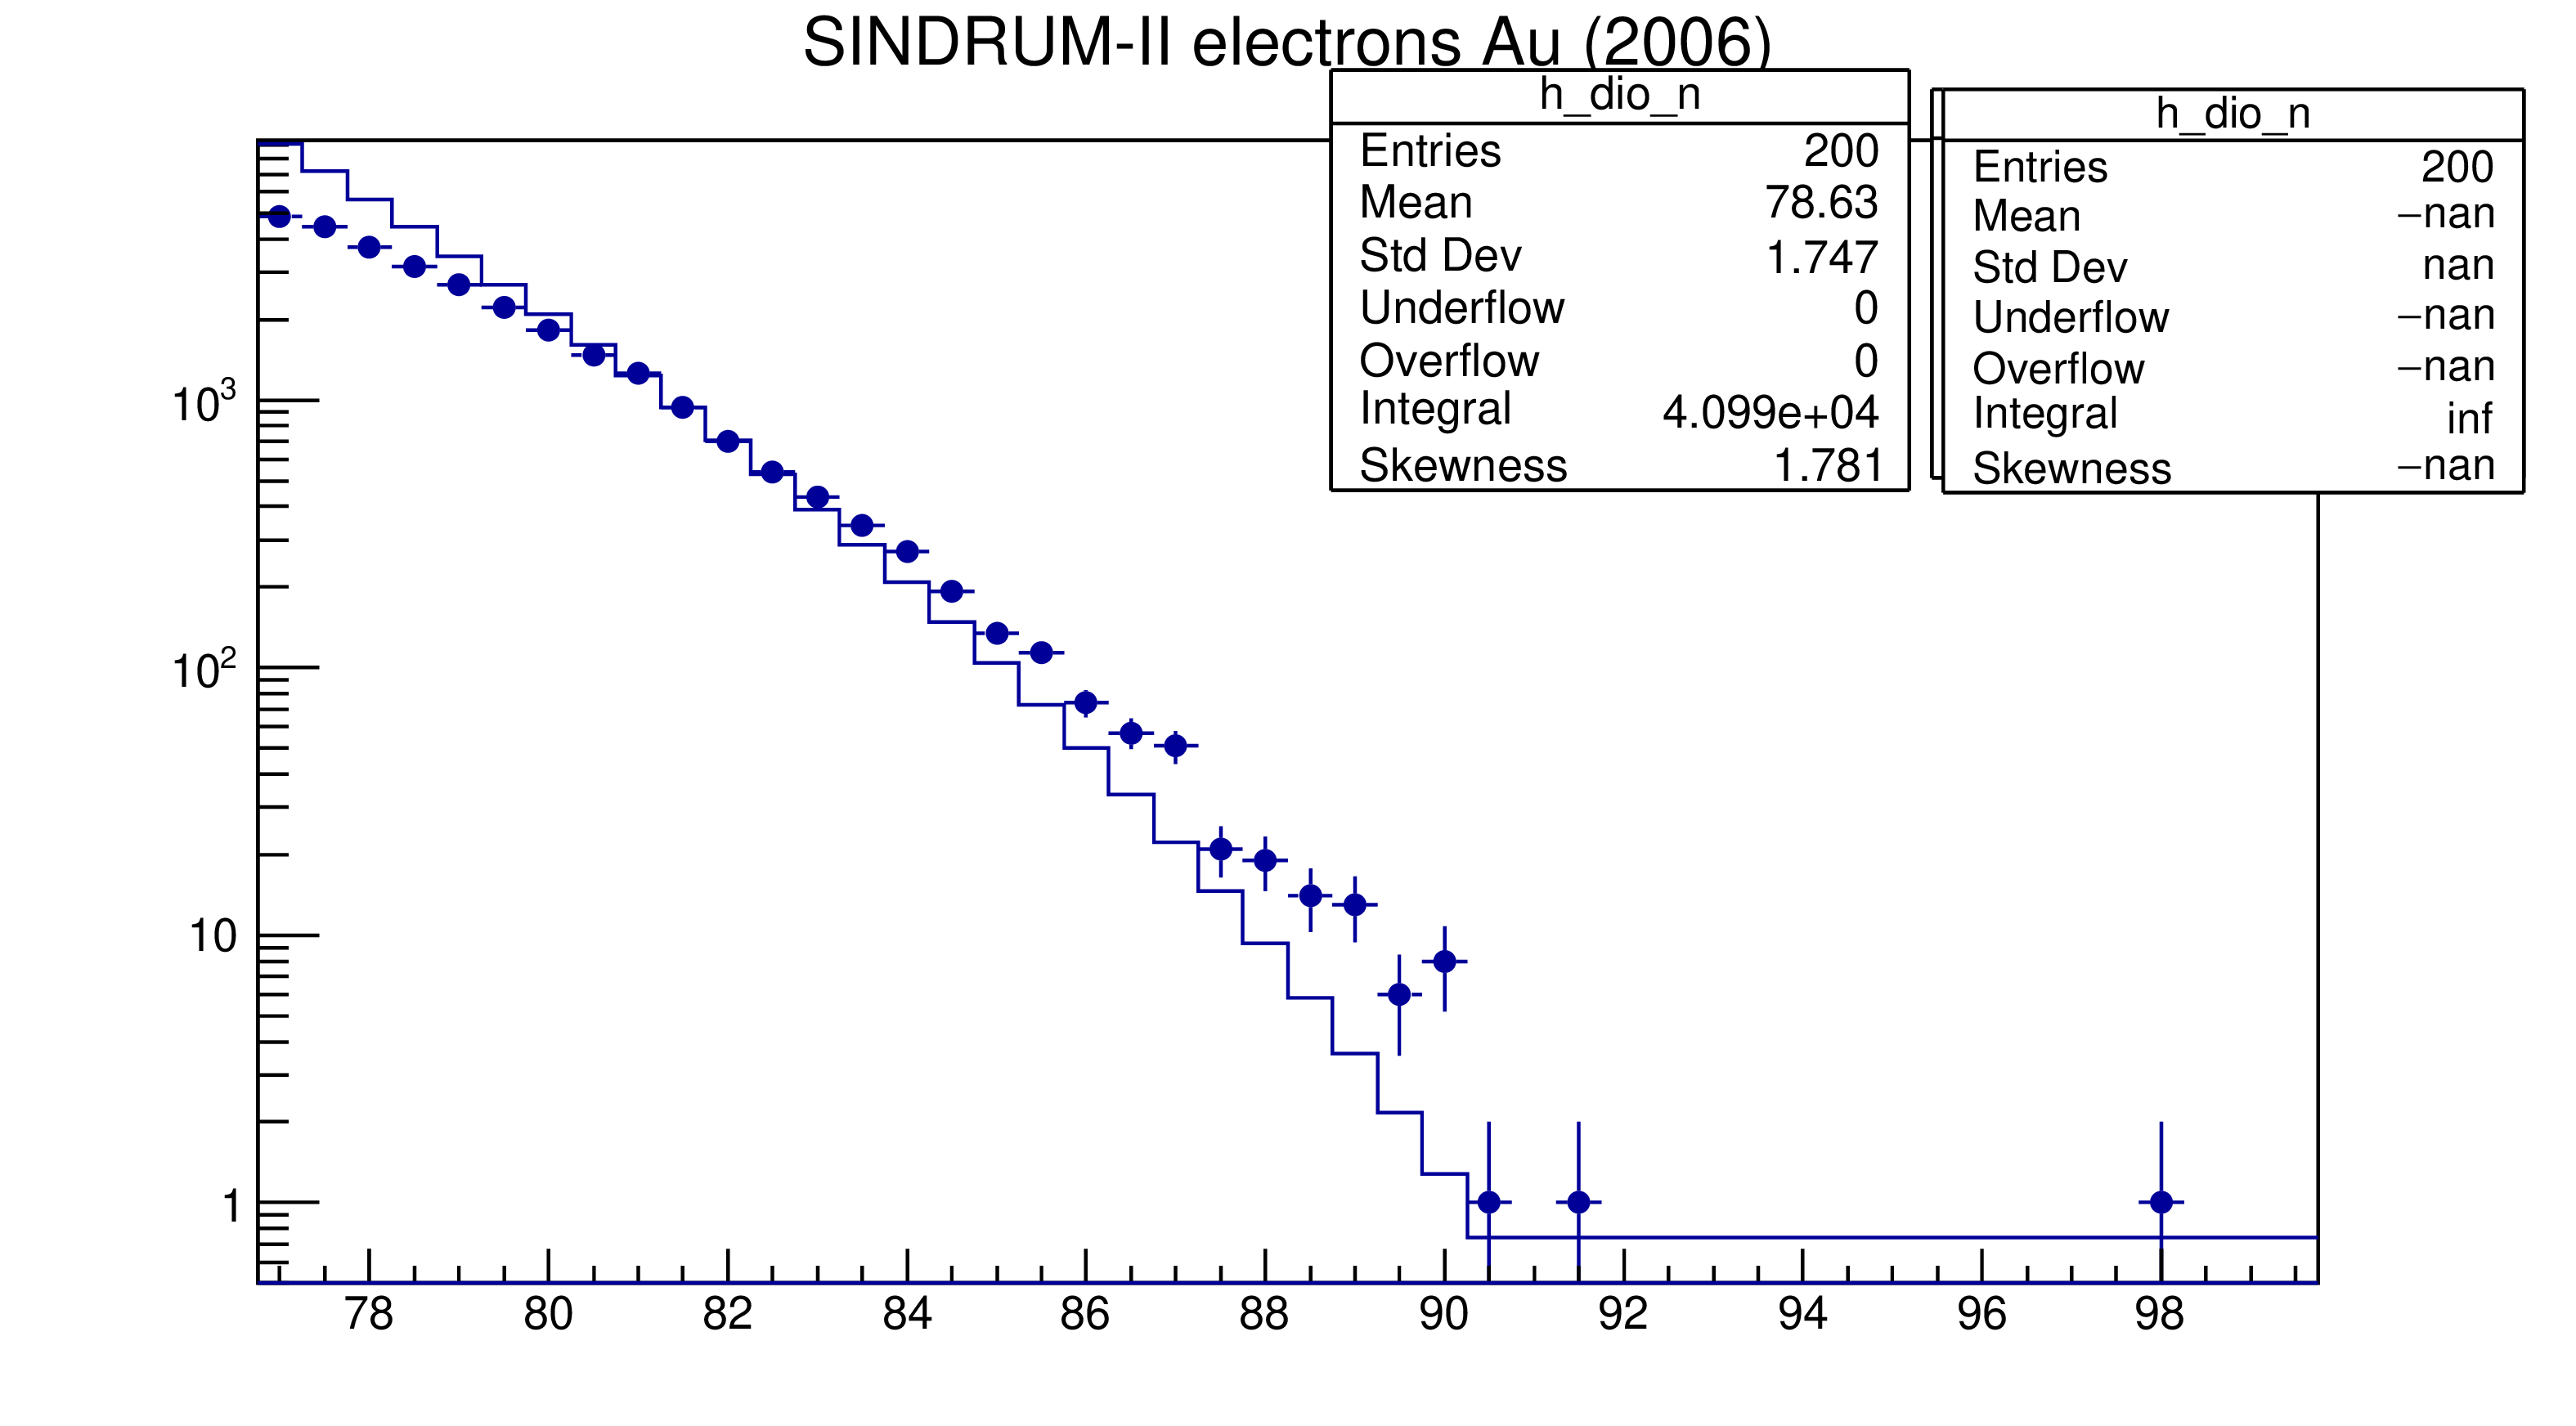
\includegraphics[width=0.99\textwidth]{figures/png/ana_step1_dio_normalized_above_80}
    }
  };
  % \node [text width=6cm, scale=0.8] at (4.5,6.4) {mu2e-18894 by Kevin Lynch and Jim Popp};
\end{tikzpicture}

placeholder
\begin{tikzpicture}
  \node[anchor=south west,inner sep=0] at (0,0.) {
    % \node[shift={(0 cm,0.cm)},inner sep=0,rotate={90}] at (0,0) {}
    \makebox[\textwidth][c] {
      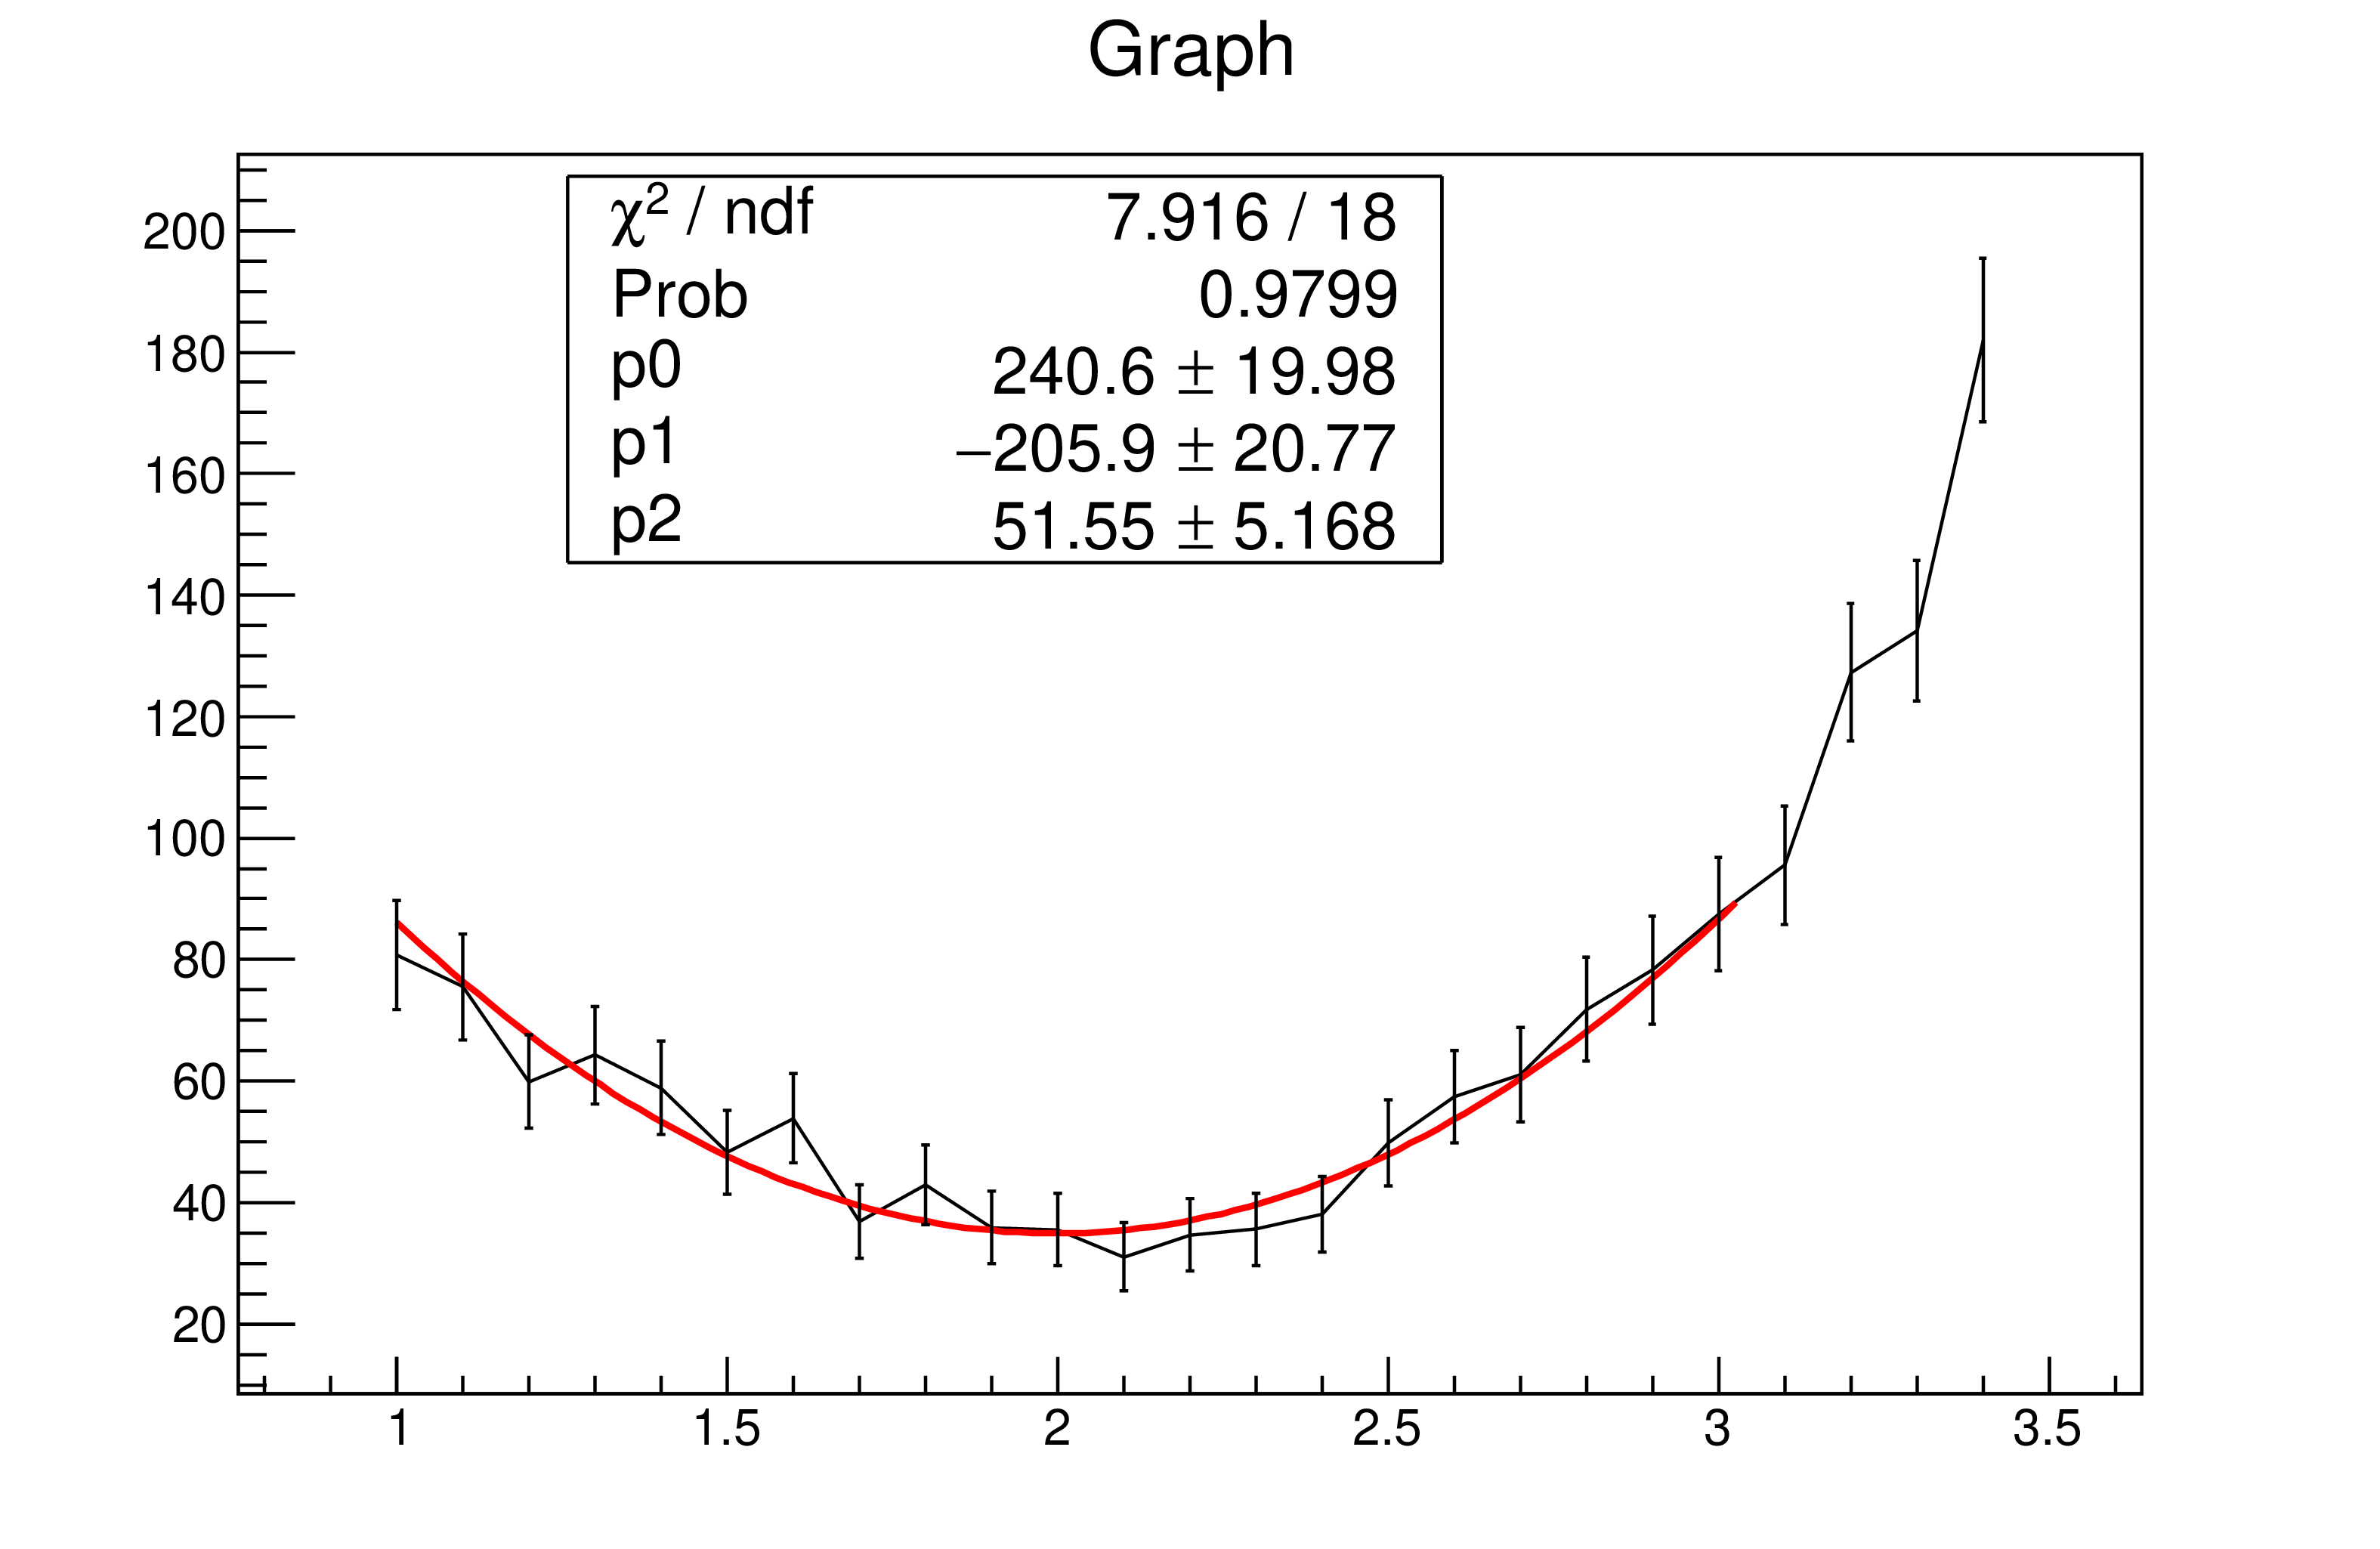
\includegraphics[width=0.99\textwidth]{figures/png/ana_step1_fit_sigma}
    }
  };
  % \node [text width=6cm, scale=0.8] at (4.5,6.4) {mu2e-18894 by Kevin Lynch and Jim Popp};
\end{tikzpicture}
